\chapter{Assembling the frame vertex triangles}
	\section{}
	Take one of the 370mm threaded rods, and slip an M8 washer onto the middle of
	it. \\
	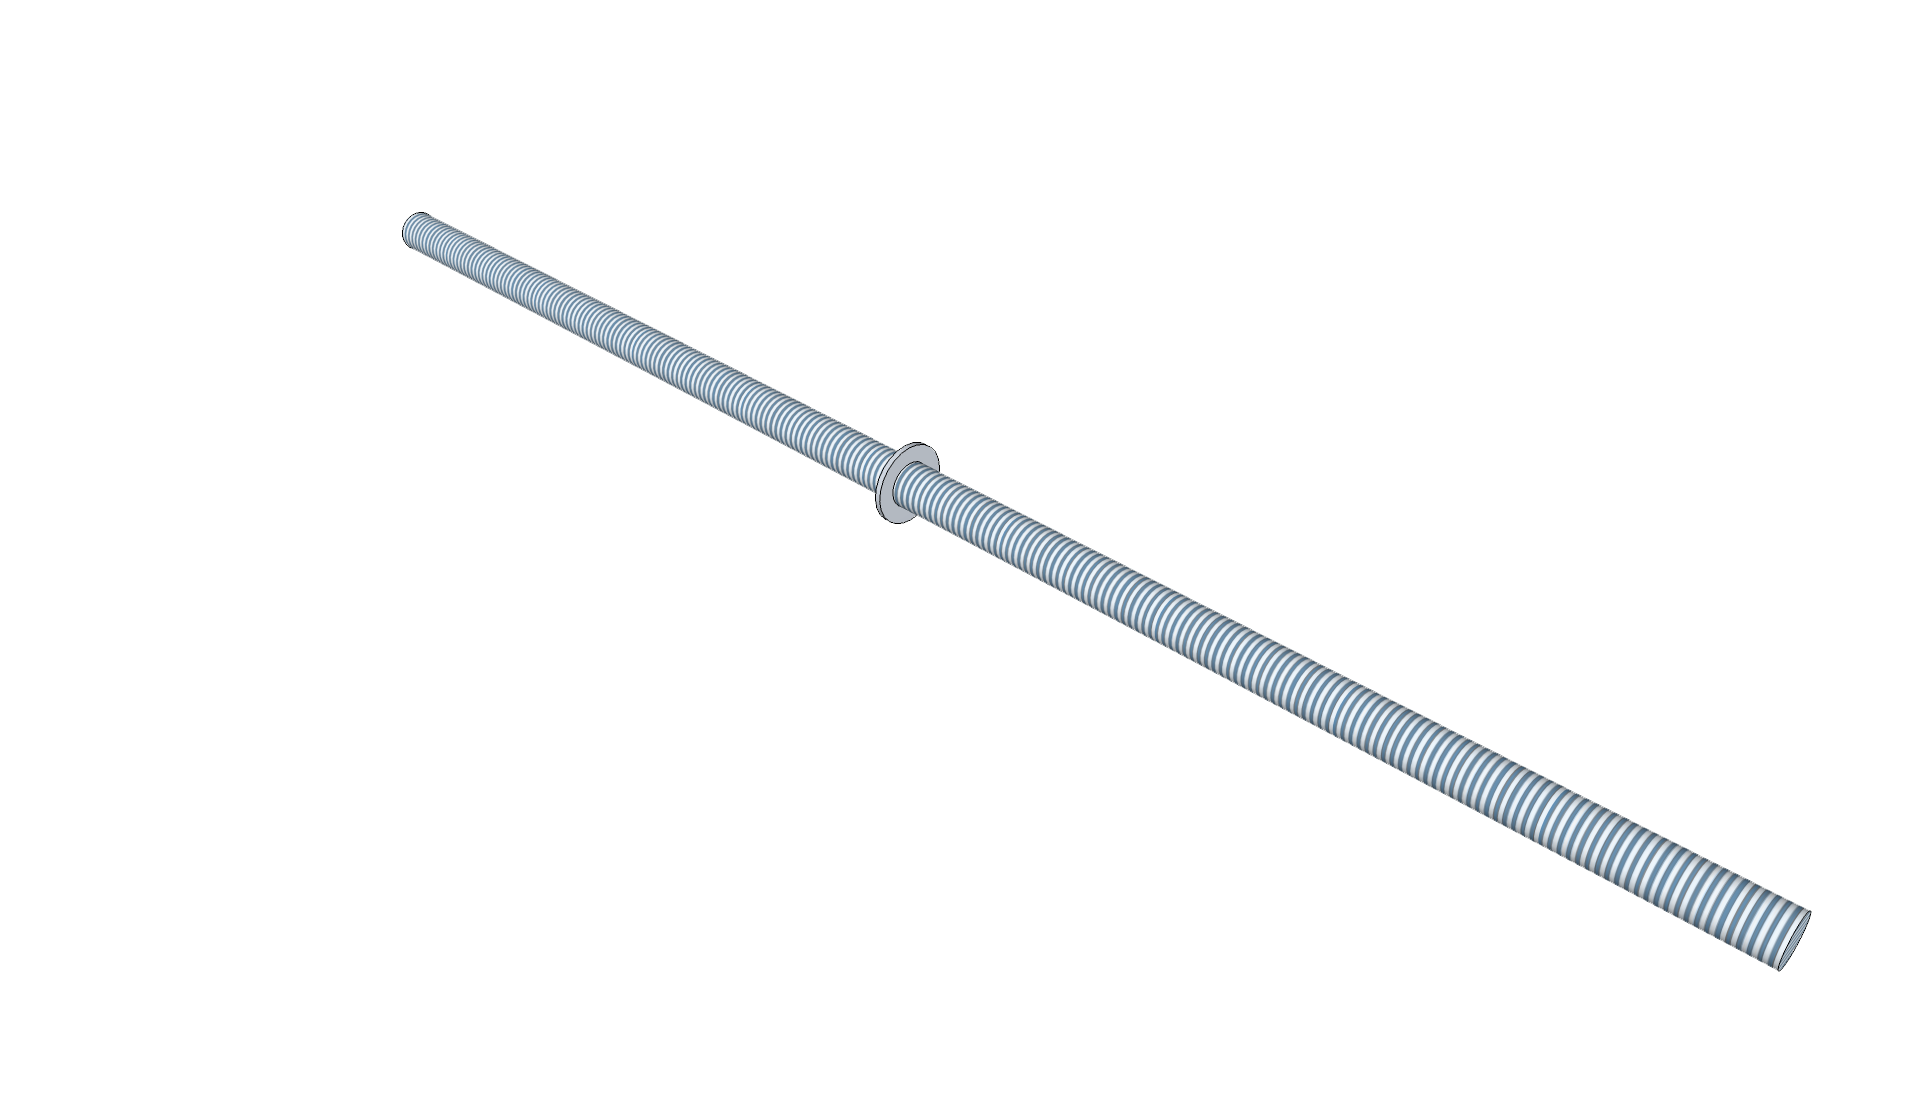
\includegraphics[width=1\linewidth]{graphics/ch1_1.png}
	
	\section{}
	Take the RP bar clamp (the U-shaped bit with the two holes) and slide the threaded rod through the two
	holes until the clamp sits next to the washer. \\
	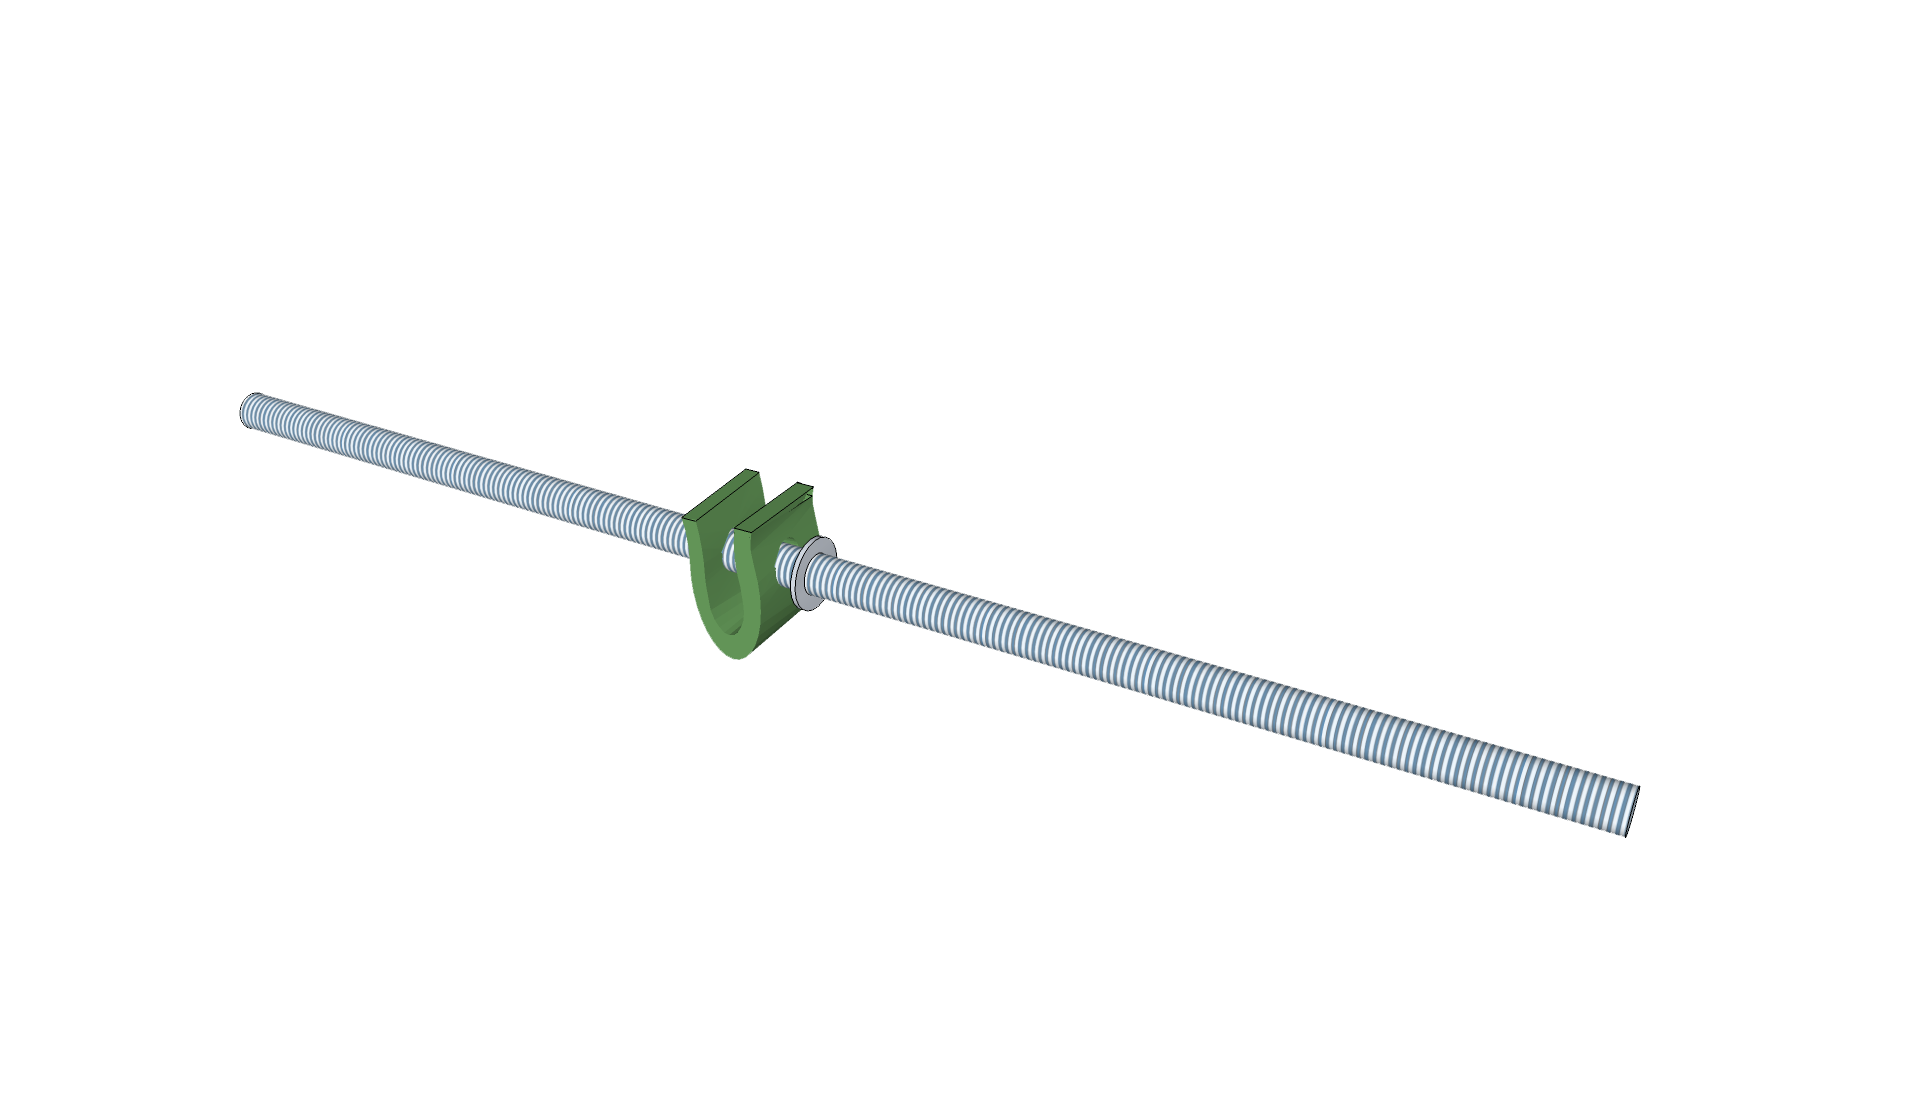
\includegraphics[width=1\linewidth]{graphics/ch1_2.png}
	
	\section{}
	Slide another washer onto the rod from the other side. \\
	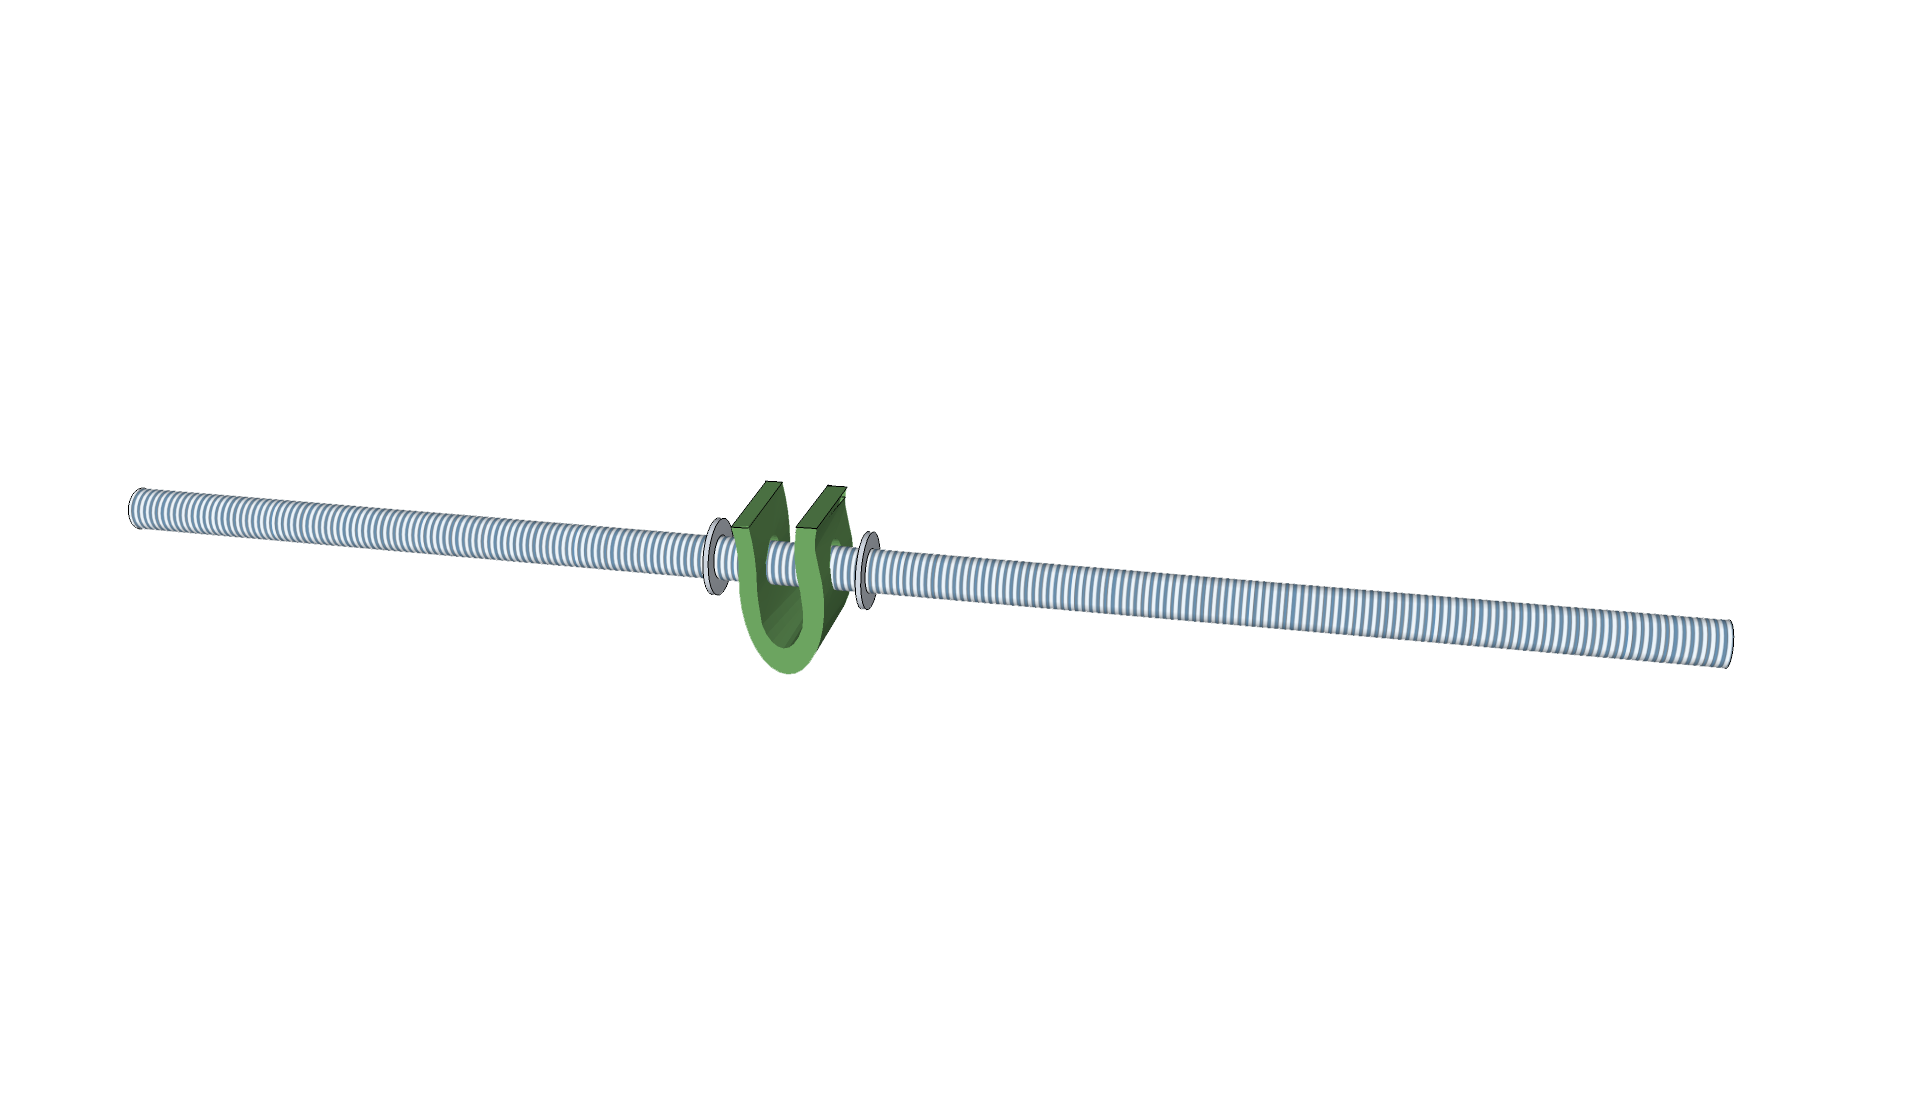
\includegraphics[width=1\linewidth]{graphics/ch1_3.png}
	
	\section{}
	Thread two M8 nuts onto either side of the clamp, until they are next to the washer, but do not tighten
	them yet. \\
	\begin{overpic}[width=1\linewidth]{graphics/ch1_4_1.png}
		\put(0,0){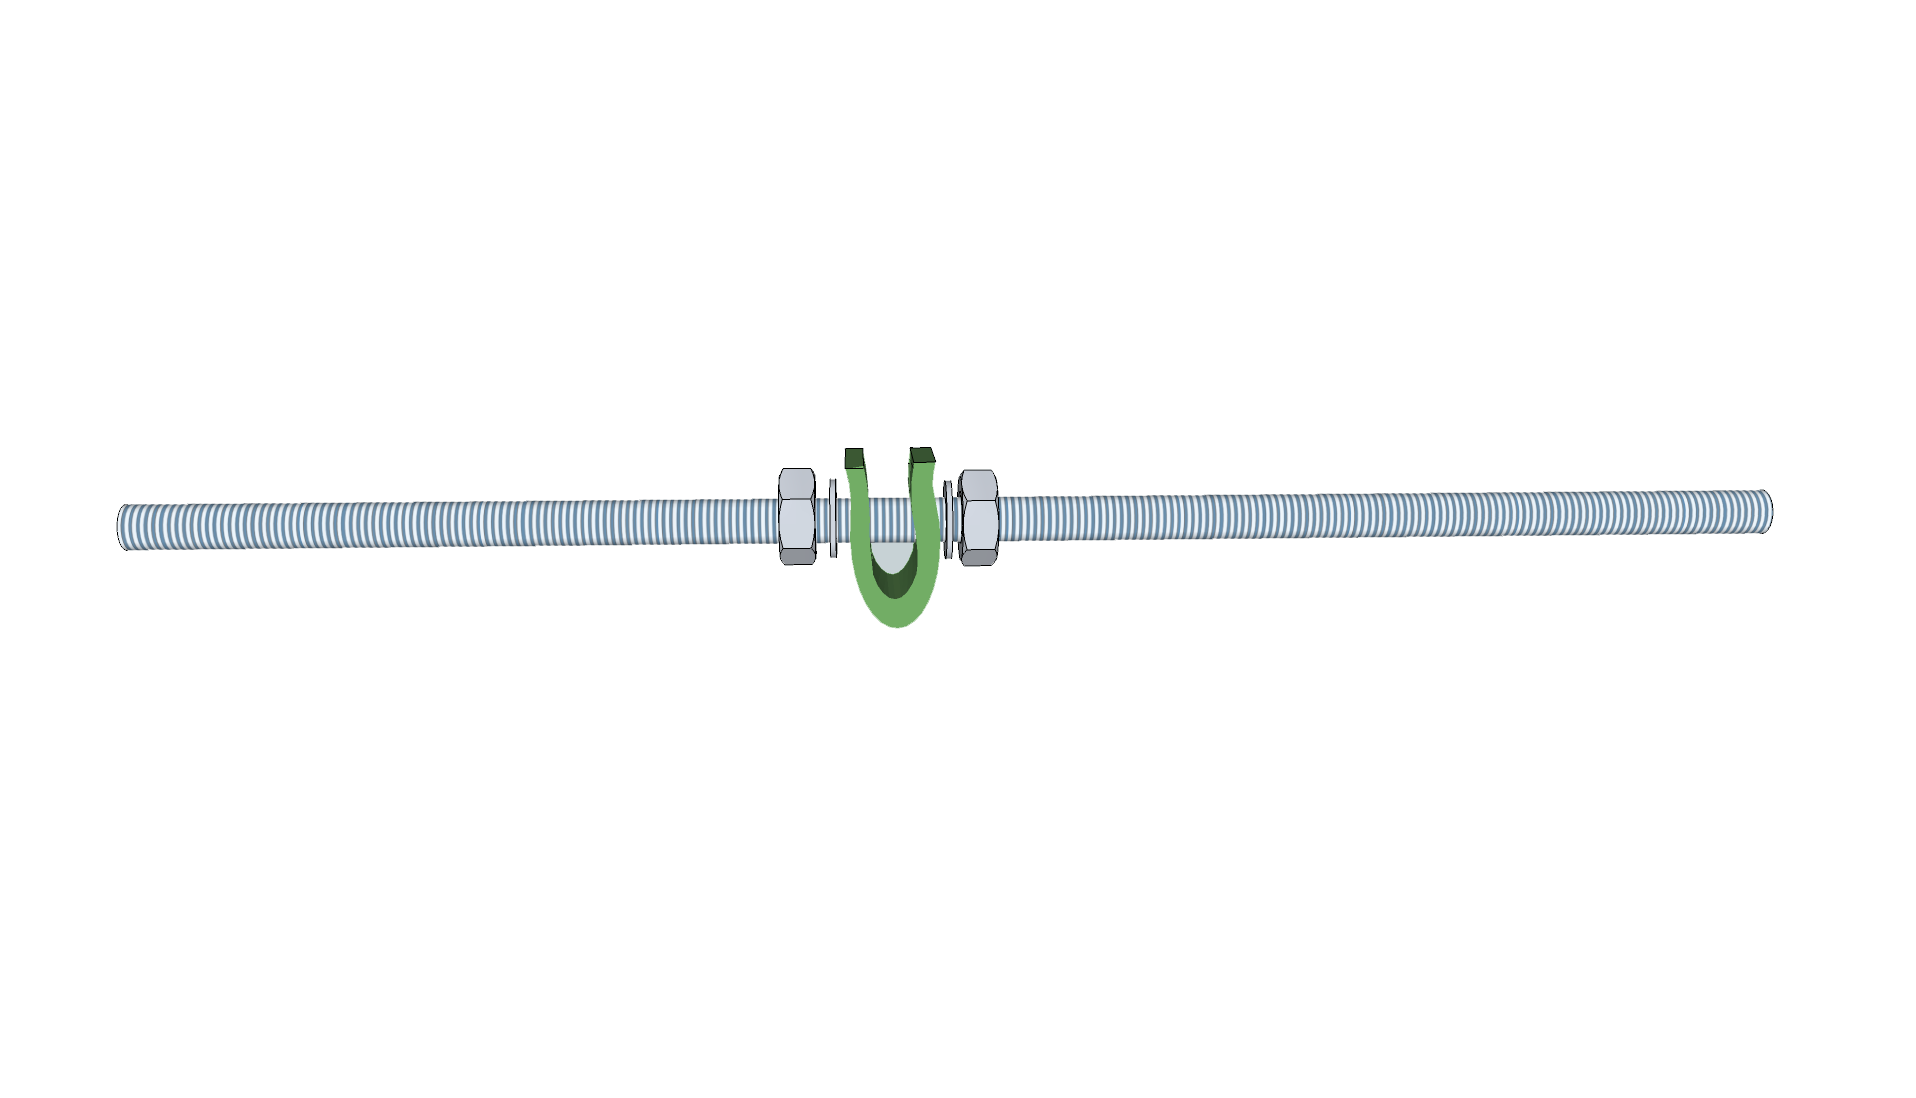
\includegraphics[width=0.4\linewidth]{graphics/ch1_4_2.png}}
	\end{overpic}
	
	\section{}
	Thread another two nuts on each side of the rod, followed by washers. See the picture for what it
	should look like. \\
	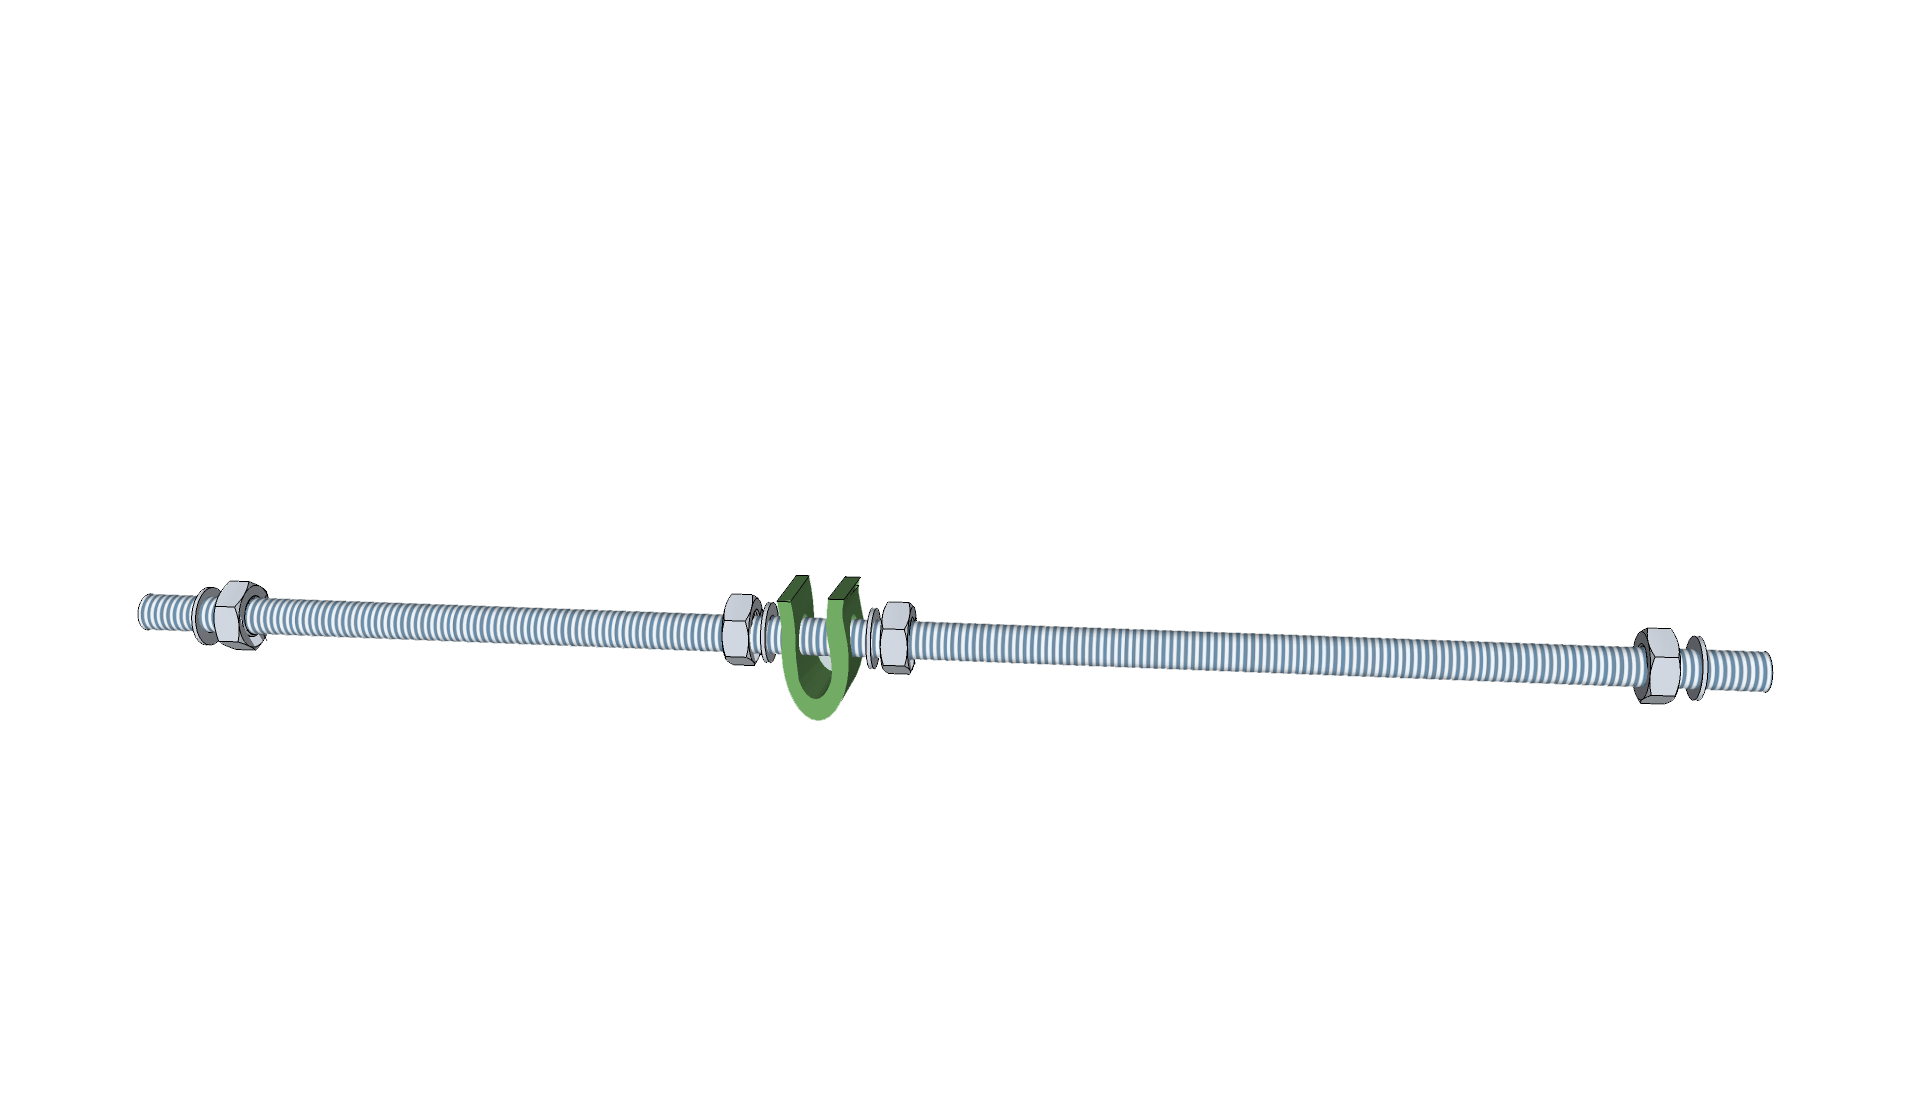
\includegraphics[width=1\linewidth]{graphics/ch1_5.png}
	
	\section{}
	Slide the rod through the long bottom (footed) side of two vertices. Make sure the feet point in the same
	direction. Also make sure the bulge on the non-footed side of the vertex points
	outwards. \\
	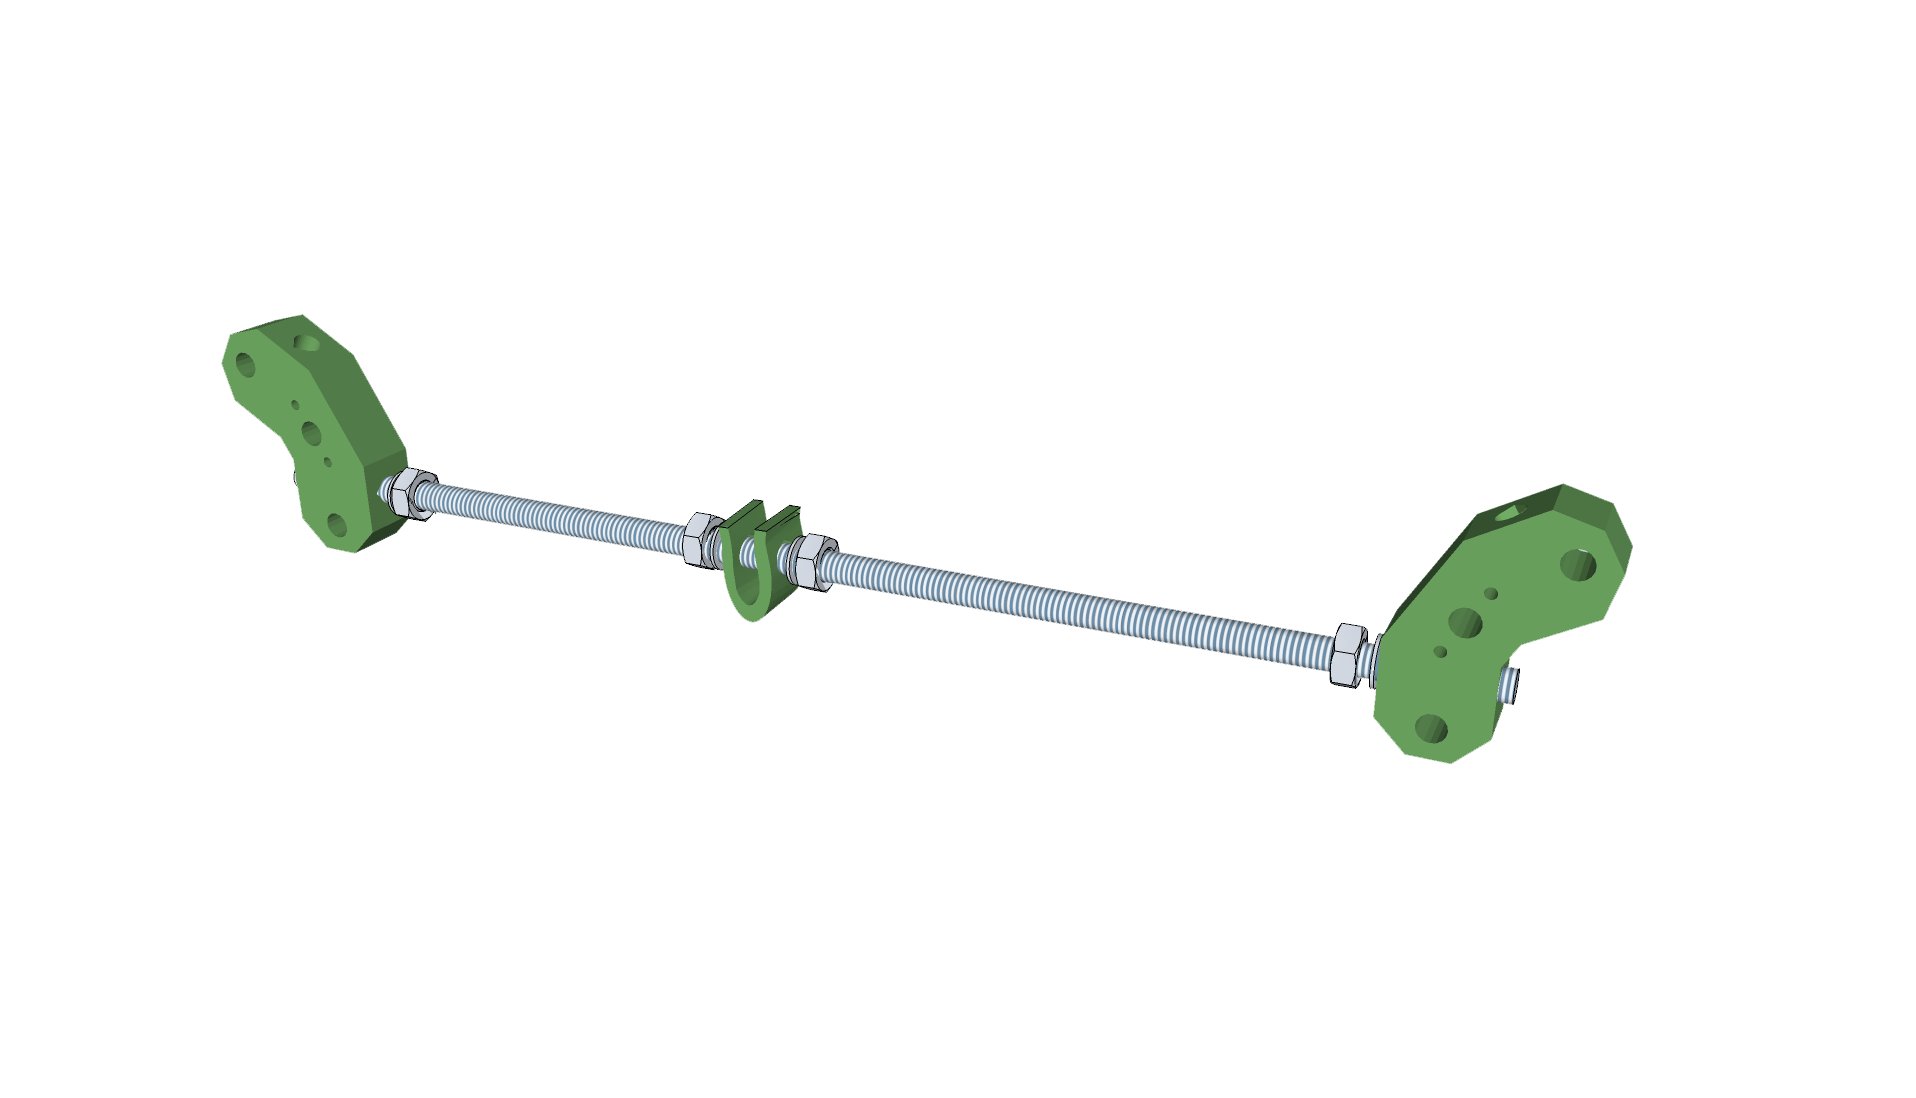
\includegraphics[width=1\linewidth]{graphics/ch1_6_1.png} \\
	You can use either footed or non-footed vertices to build this (the footed ones
	look better, but are not critical.) \\
	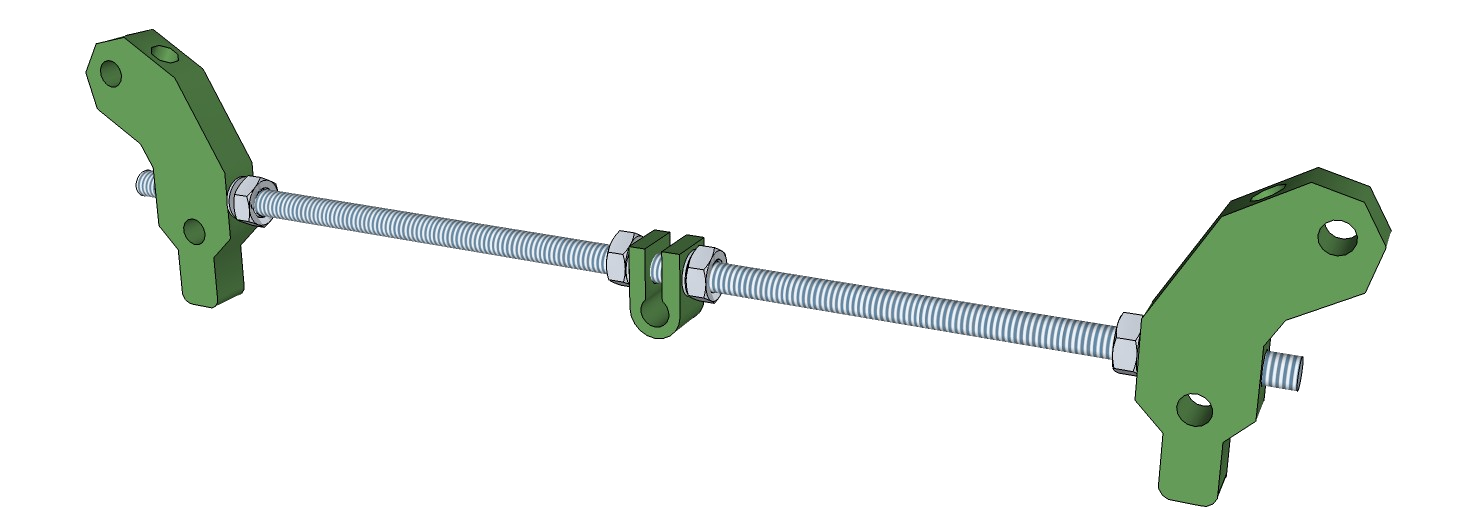
\includegraphics[width=1\linewidth]{graphics/ch1_6_2.png}
	
	\section{}
	Measure the distance. The distance between the two vertices should be 290mm (along the rod,
	equivalent is 11-13/32"). Get it approximately right now, we will check this again later. If you have a
	frame jig, place it between the two vertices and adjust the nuts until you can just barely fit the jig J1
	between them. \\
	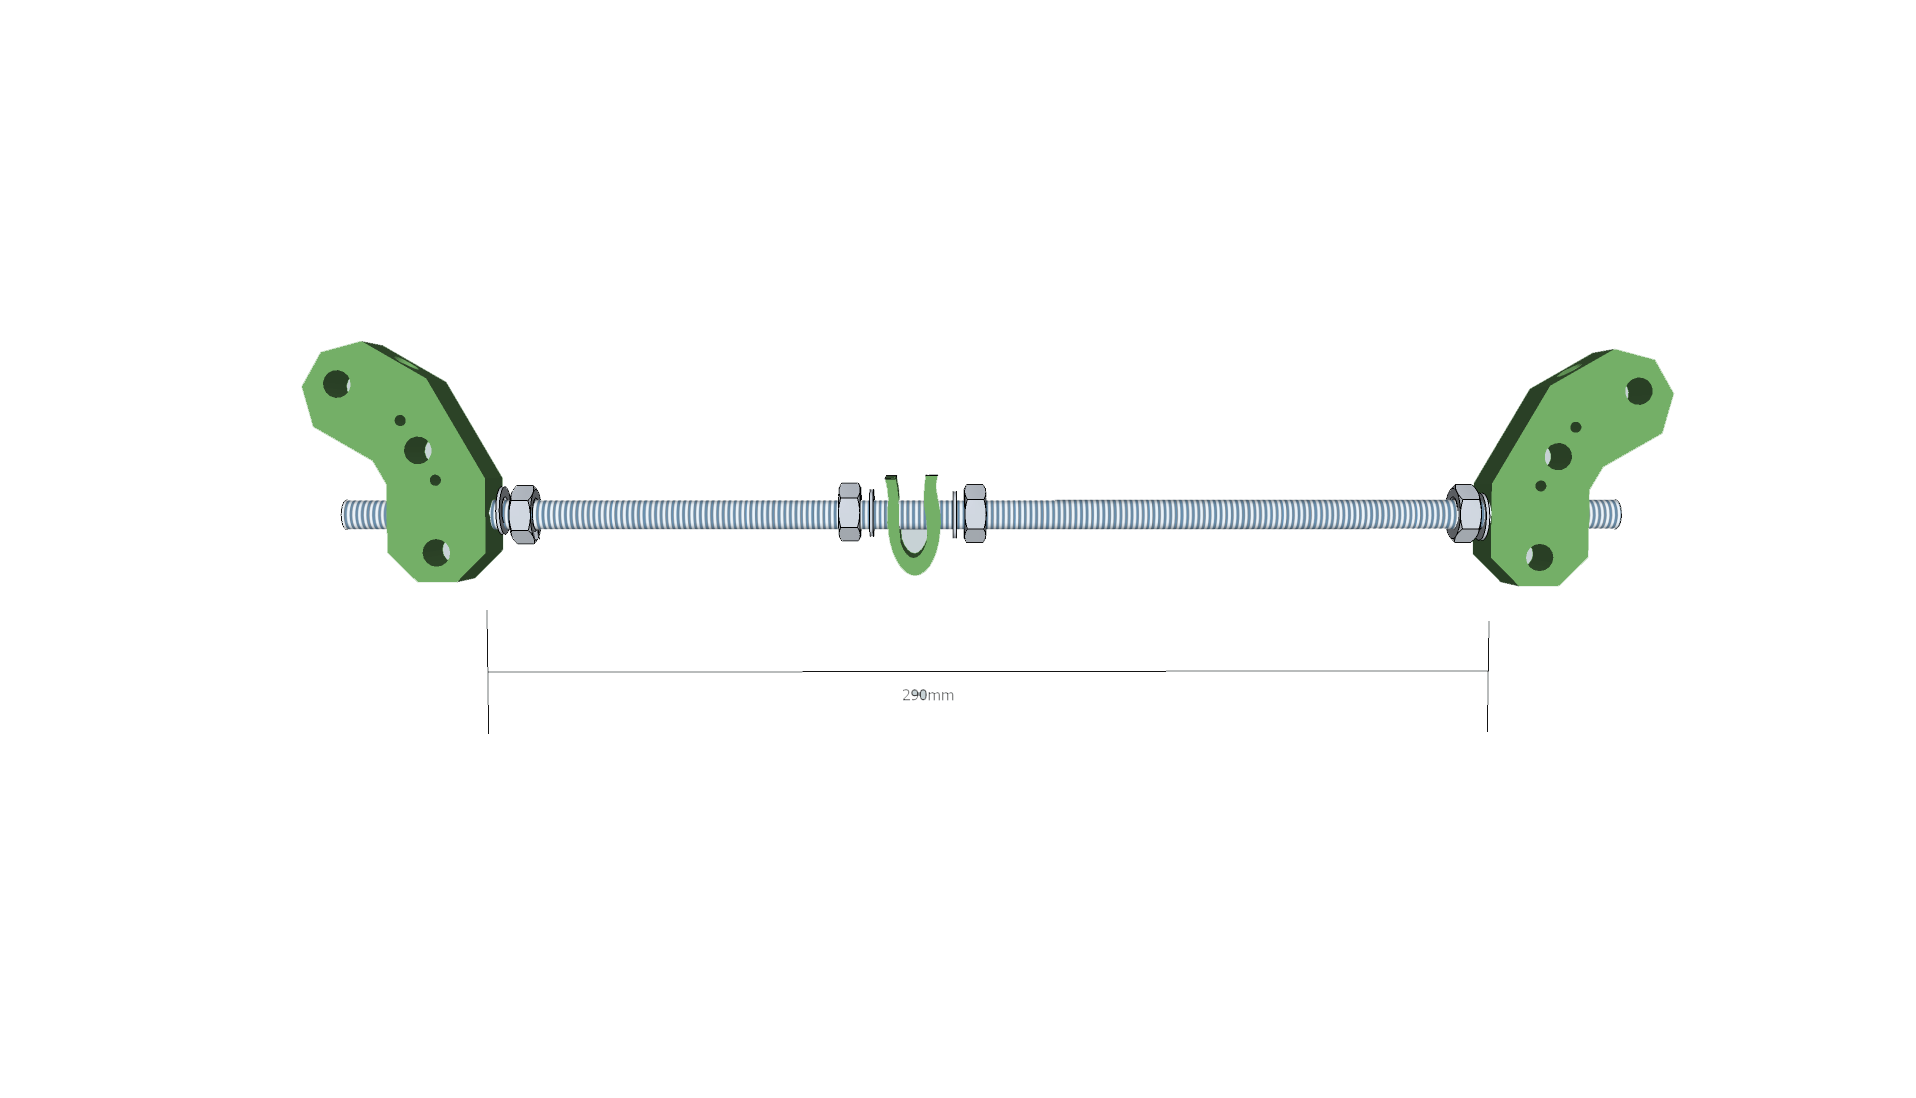
\includegraphics[width=1\linewidth]{graphics/ch1_7.png}
	
	\section{}
	Place another washer and nut on the other side of the vertex. Tighten, but not too much. We'll need a
	bit of flexibility here still. \\
	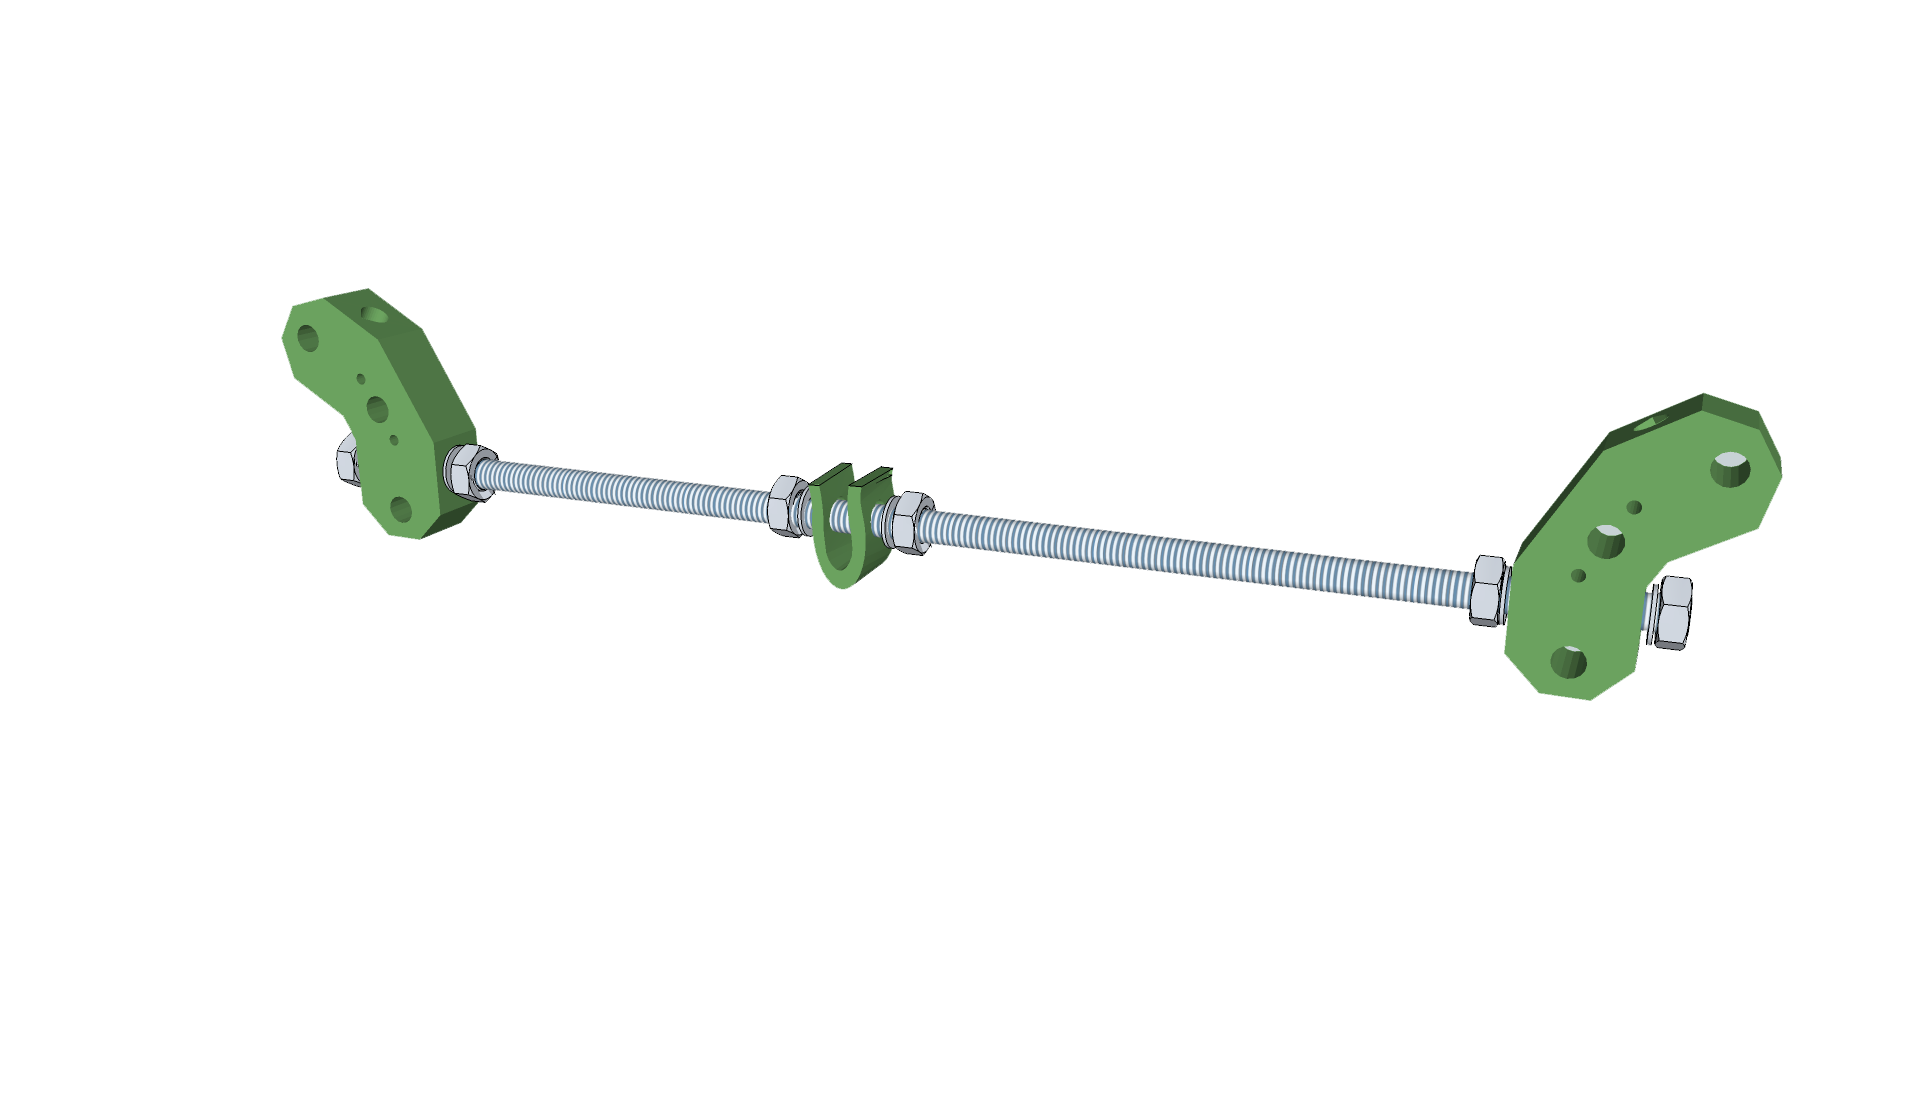
\includegraphics[width=1\linewidth]{graphics/ch1_8.png}
	
	\section{}
	Take another 370mm M8 threaded rod and place a nut followed by a washer at each
	end. \\
	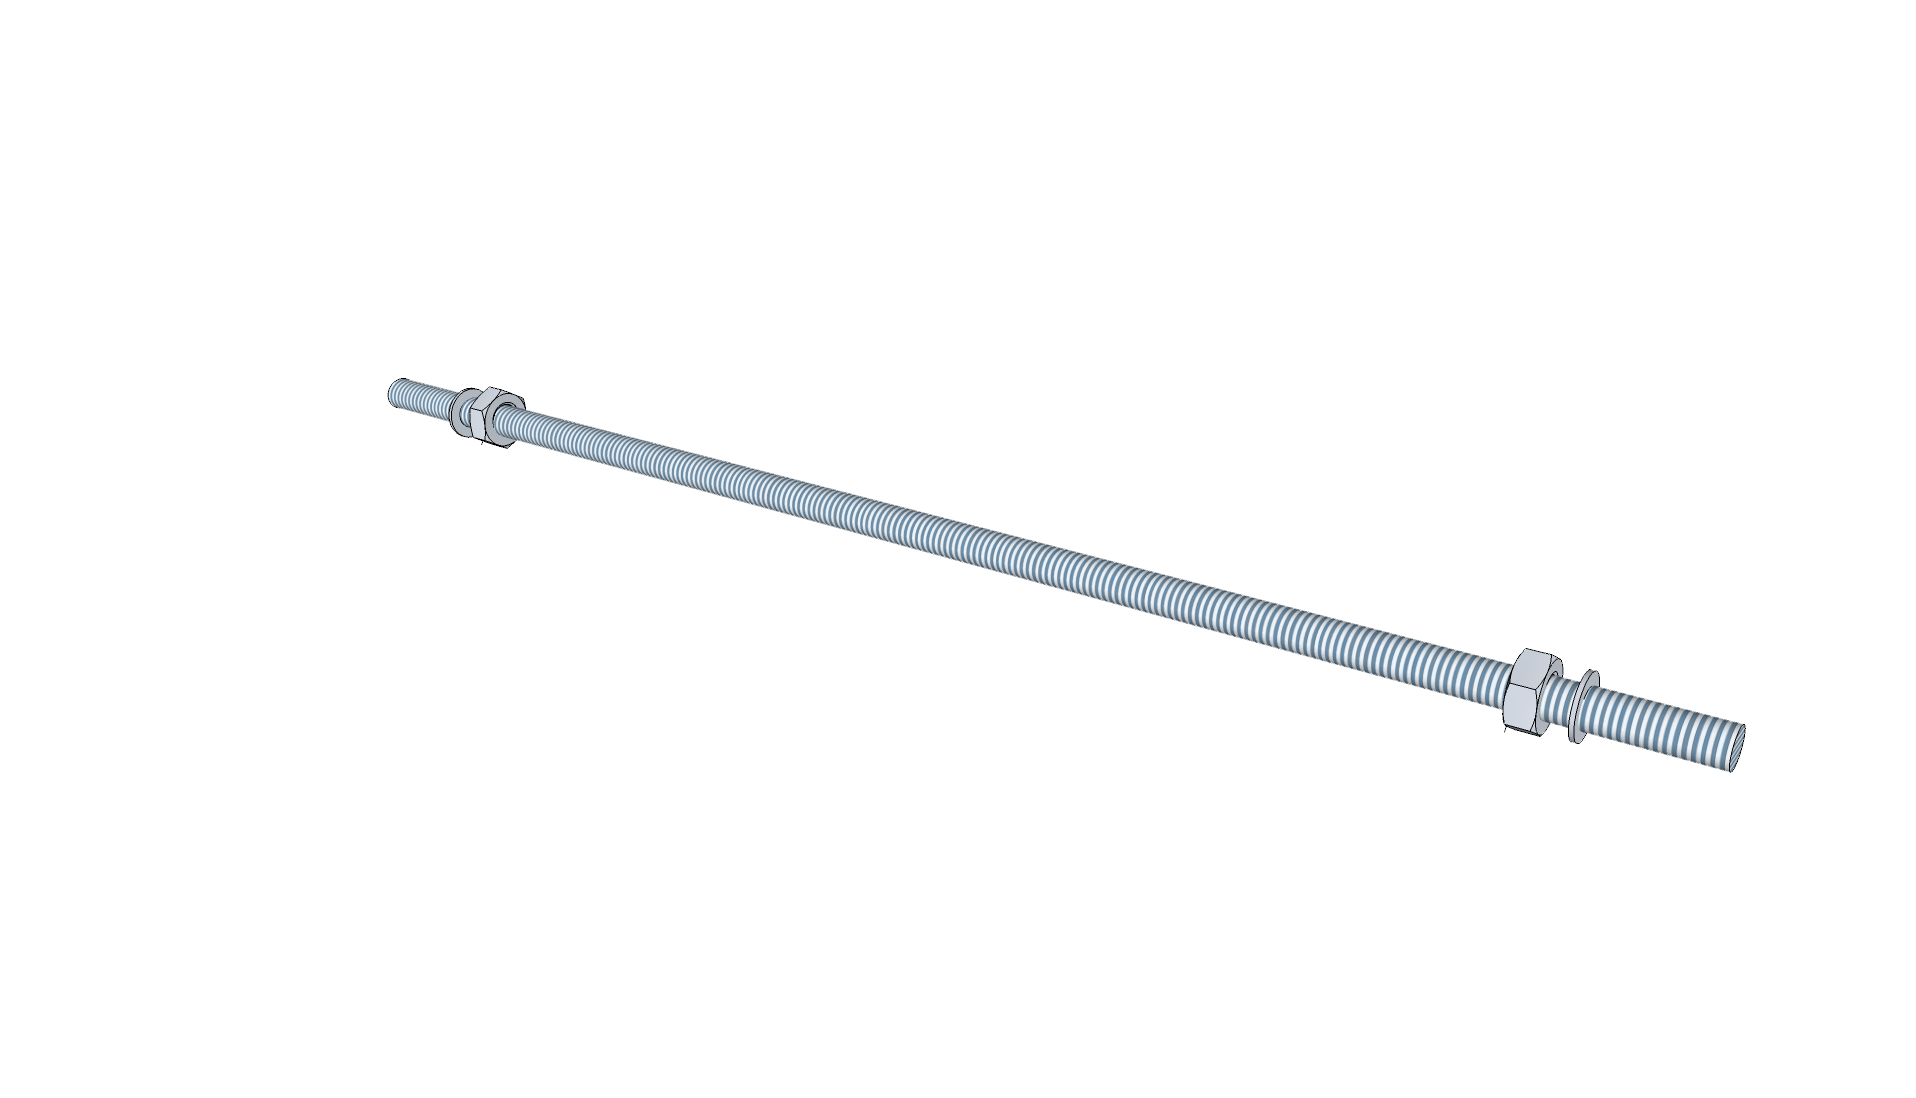
\includegraphics[width=1\linewidth]{graphics/ch1_9.png}
	
	\section{}
	Place one end of the threaded rod into the one of the two footed frame vertices. It should be in the
	same plane as the first threaded rod. Fix it in place with a washer and nut. You should now have two
	sides of the equilateral triangle.\\
	\begin{center}
		\begin{overpic}[width=1\linewidth]{graphics/ch1_10_1.png}
			\put(62,30){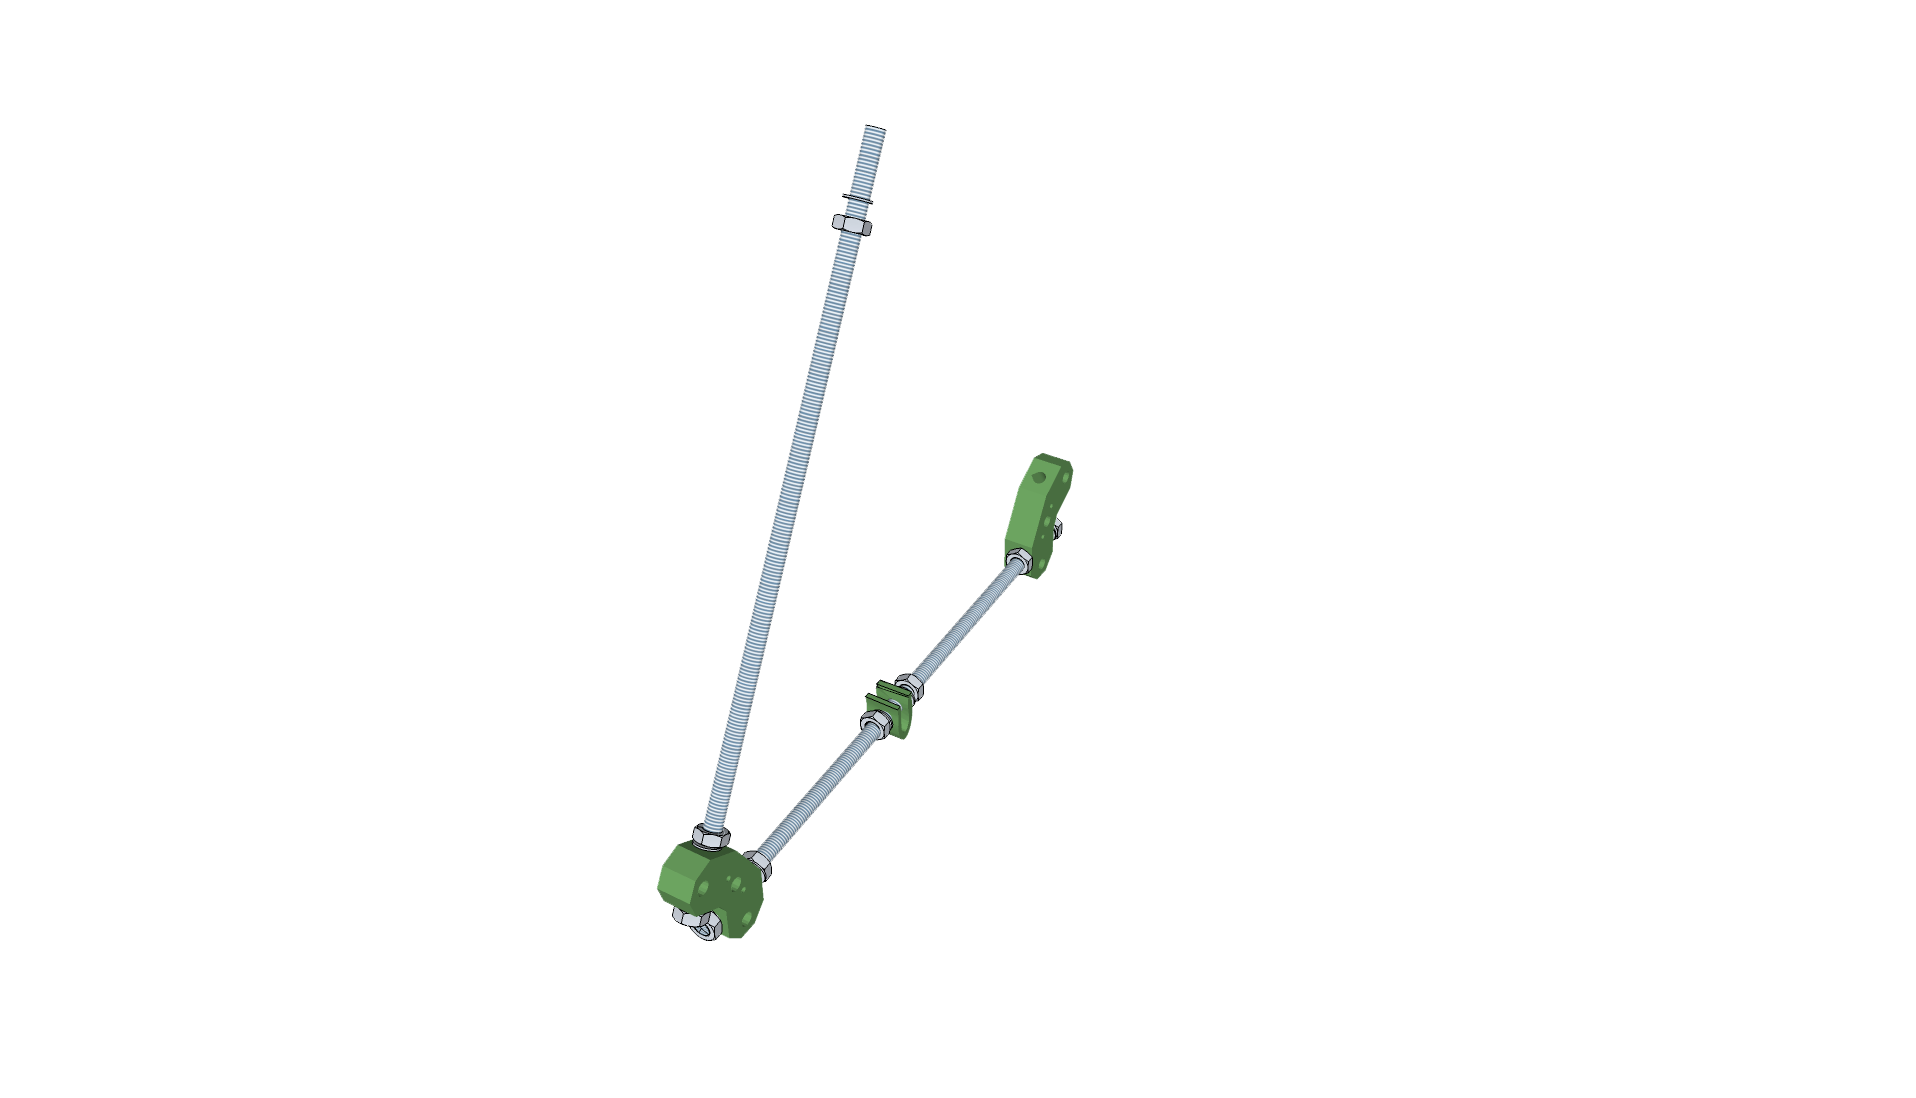
\includegraphics[width=0.5\linewidth]{graphics/ch1_10_2.png}}
		\end{overpic}
	\end{center}
	
	\section{}
	Take the third piece of threaded rod and put a nut and washer on each end. Place it in the other footed
	vertex and fix it in place with a washer and nut. You should now have a triangle of threaded rods with
	two footed vertices on two of the corners, nothing in the third corner, and a bar clamp between the two
	vertices. \\
	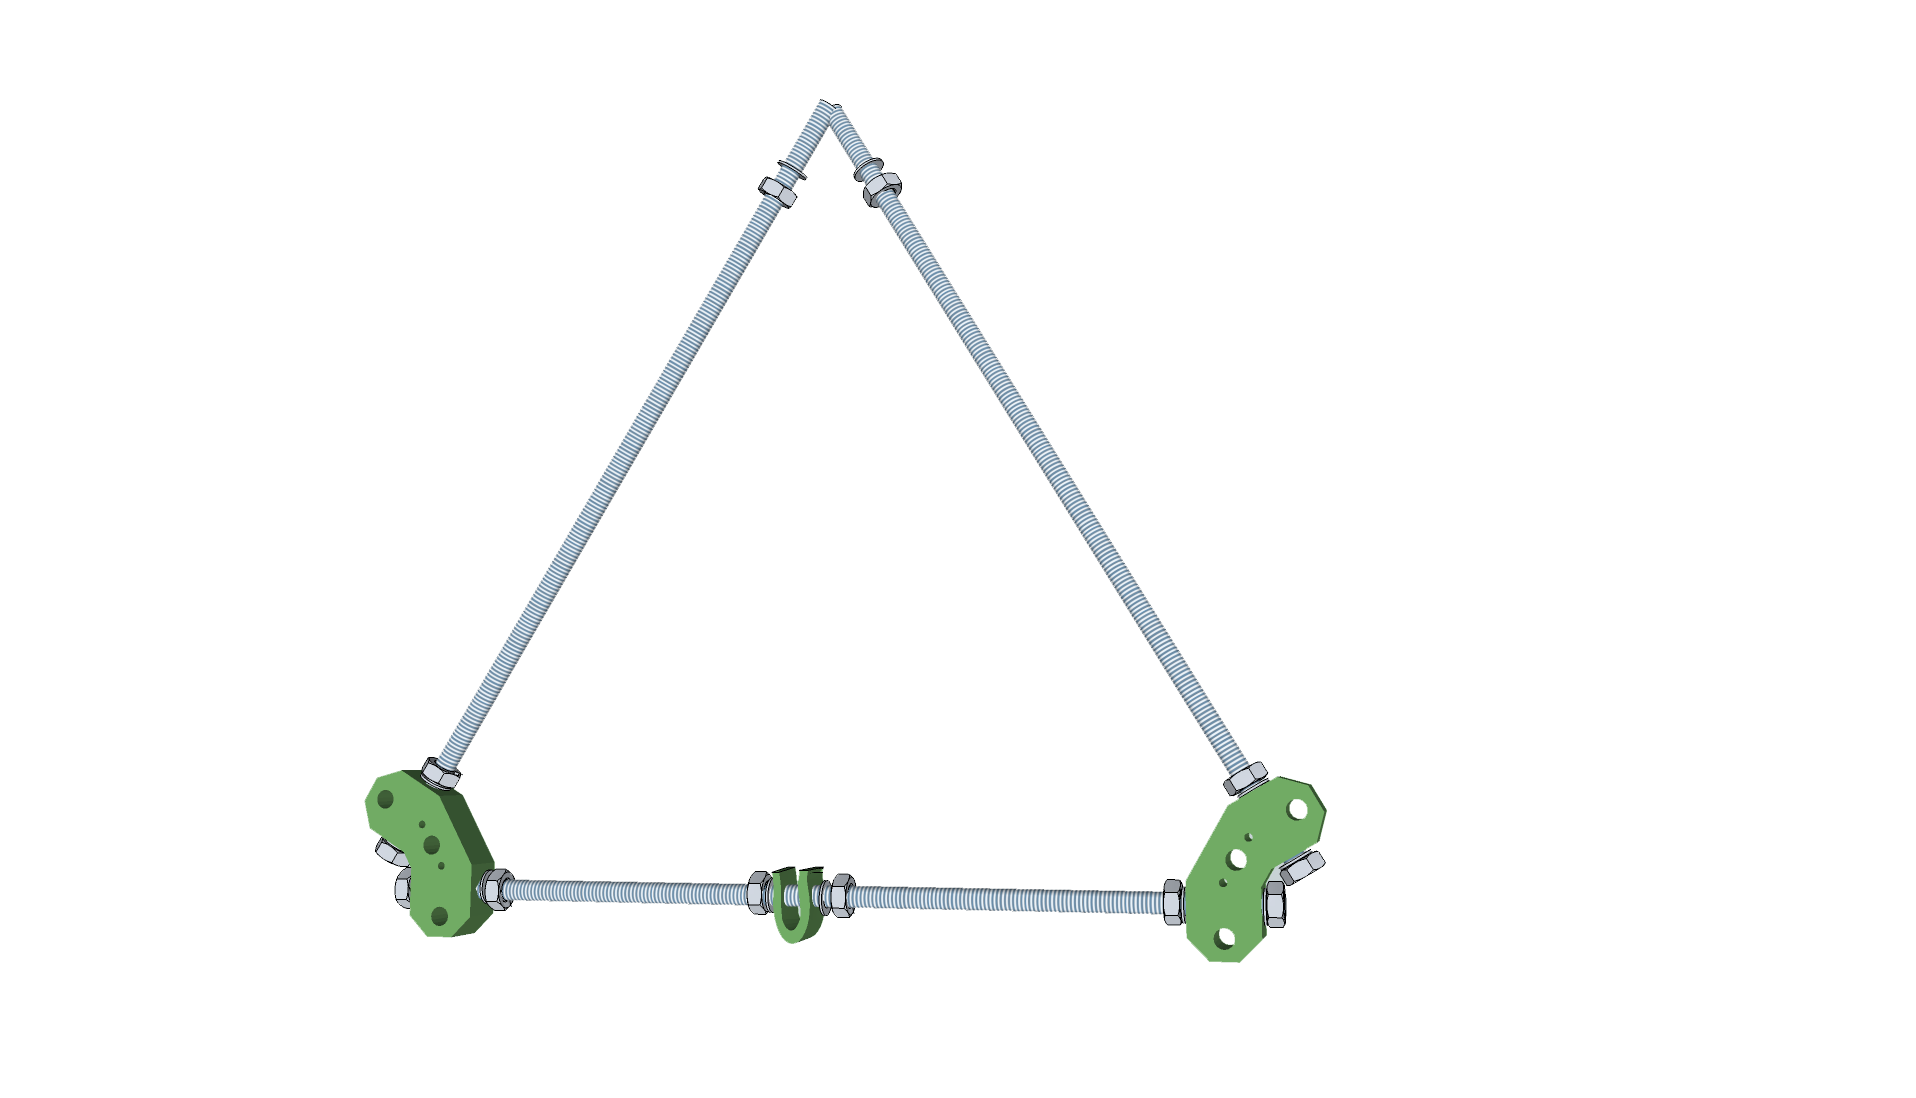
\includegraphics[width=1\linewidth]{graphics/ch1_11.png}
	
	\section{}
	Take the third vertex (non-footed) and slide it onto the threaded rods in the final corner of the triangle.
	Measure the lenghts of the three sides to make sure they are all 290mm long (along the rod from plastic
	part to plastic part, equivalent is 11-13/32"). Adjust the nuts to make sure this is so. Use the frame jig J1
	if you have one. Once done, place a washer and nut on the top of the vertex.
	Tighten all the outer nuts. \\
	\begin{center}
		\begin{overpic}[width=1\linewidth]{graphics/ch1_12_1.png}
			\put(62,30){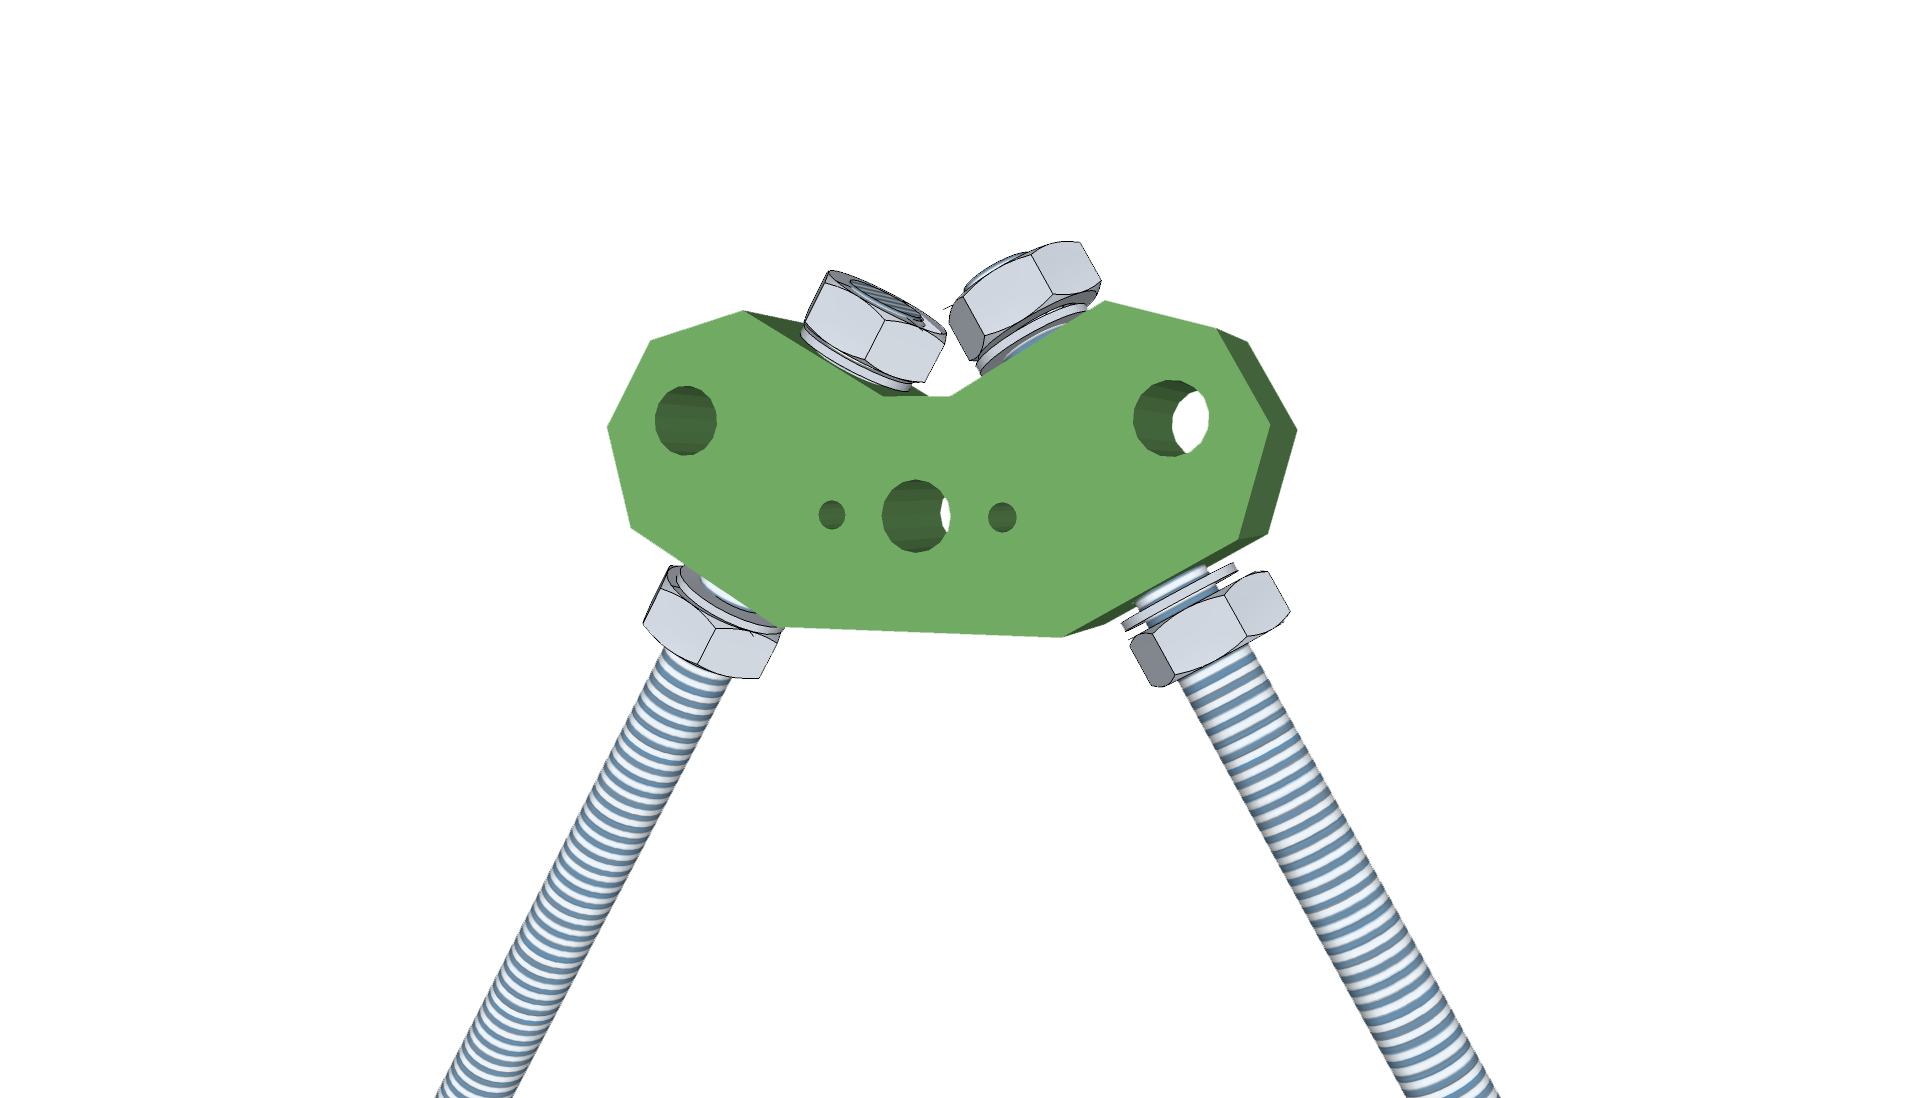
\includegraphics[width=0.5\linewidth]{graphics/ch1_12_2.png}}
		\end{overpic}
	\end{center}
	
	\section{}
	You should now have a sturdy triangle with equal-length sides, two feet on the bottom, and a bar clamp
	between the feet. Adjust the nuts around the bar clamp (but do not crush the bar clamp together yet)
	until it's approximately in the middle of the rod. Leave the nuts there loose. See photo for what you
	should have at this point. \\
	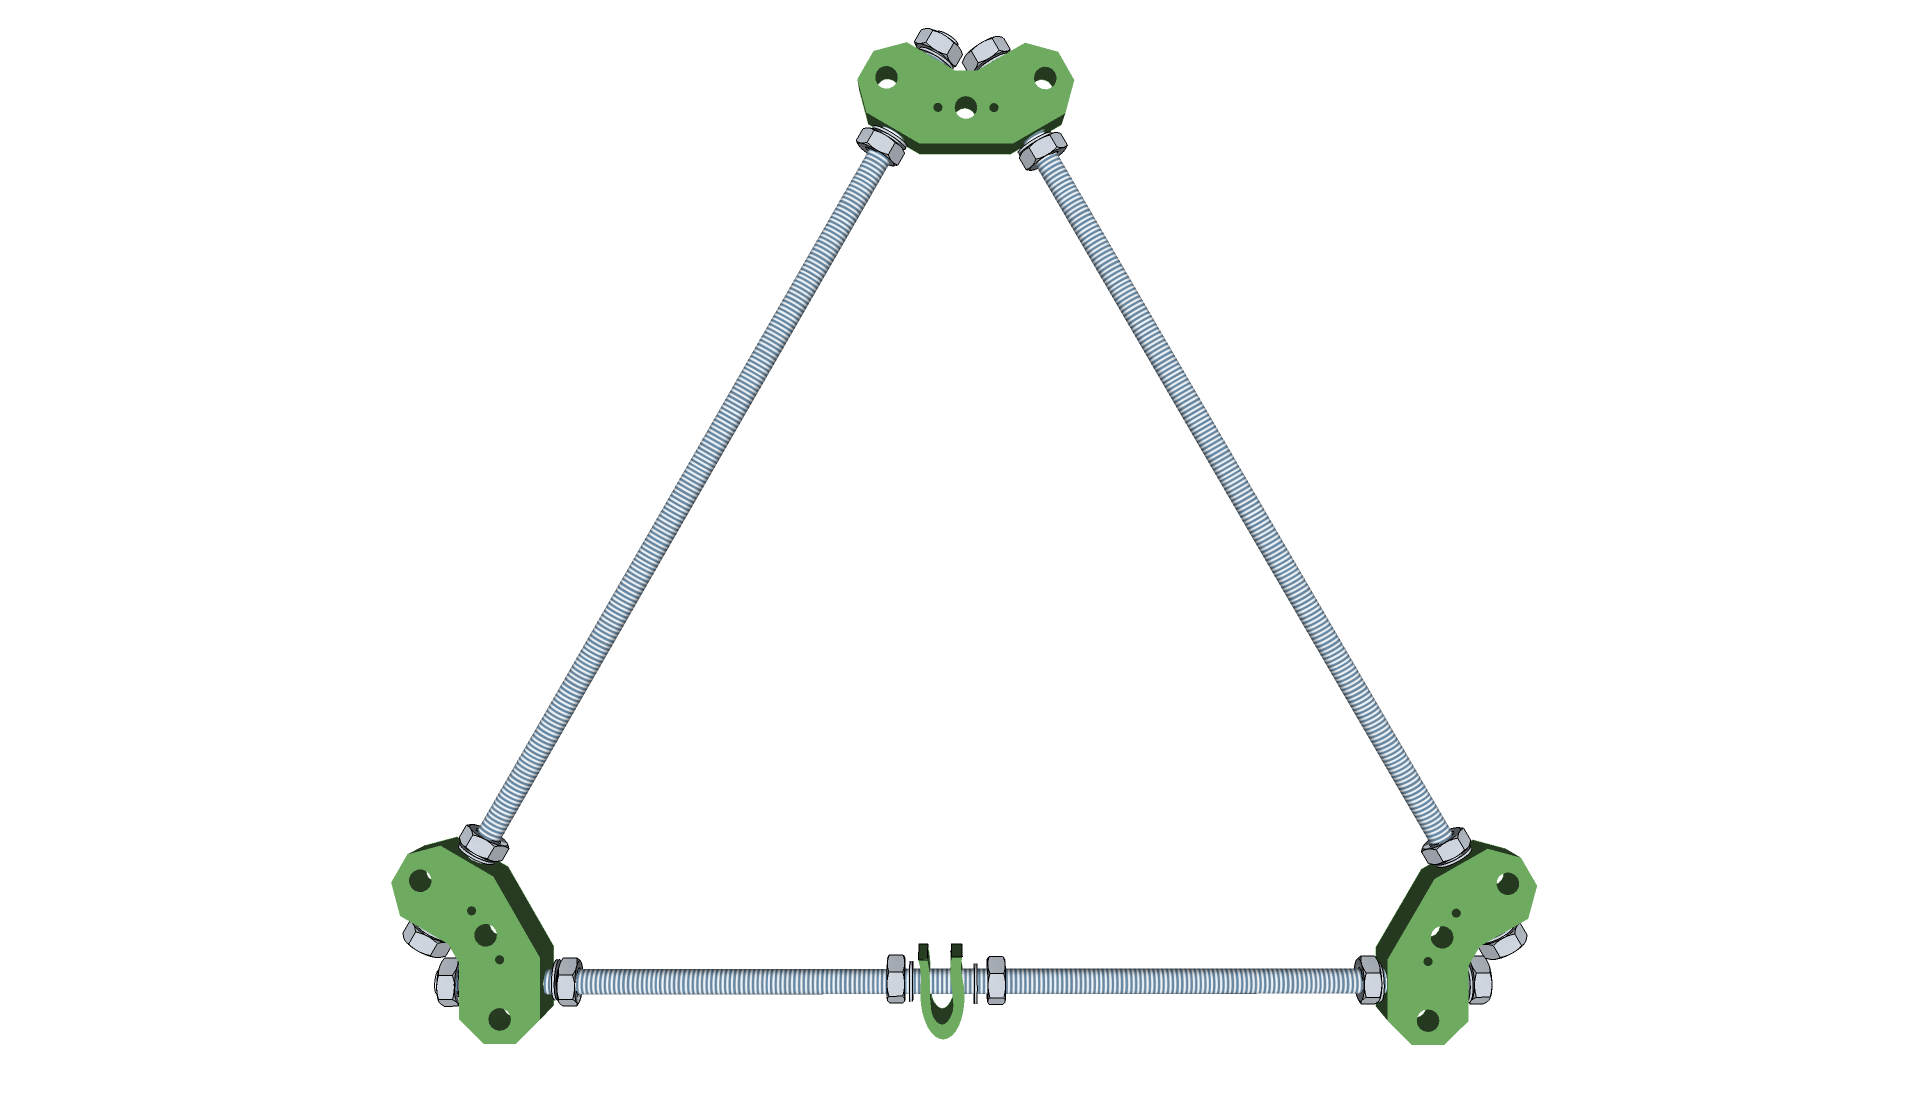
\includegraphics[width=1\linewidth]{graphics/ch1_13.png}
	
	\section{}
	That's it, that's one of the triangles done. Repeat the entire procedure for the second triangle. It is
	exactly identical to the first. \\
	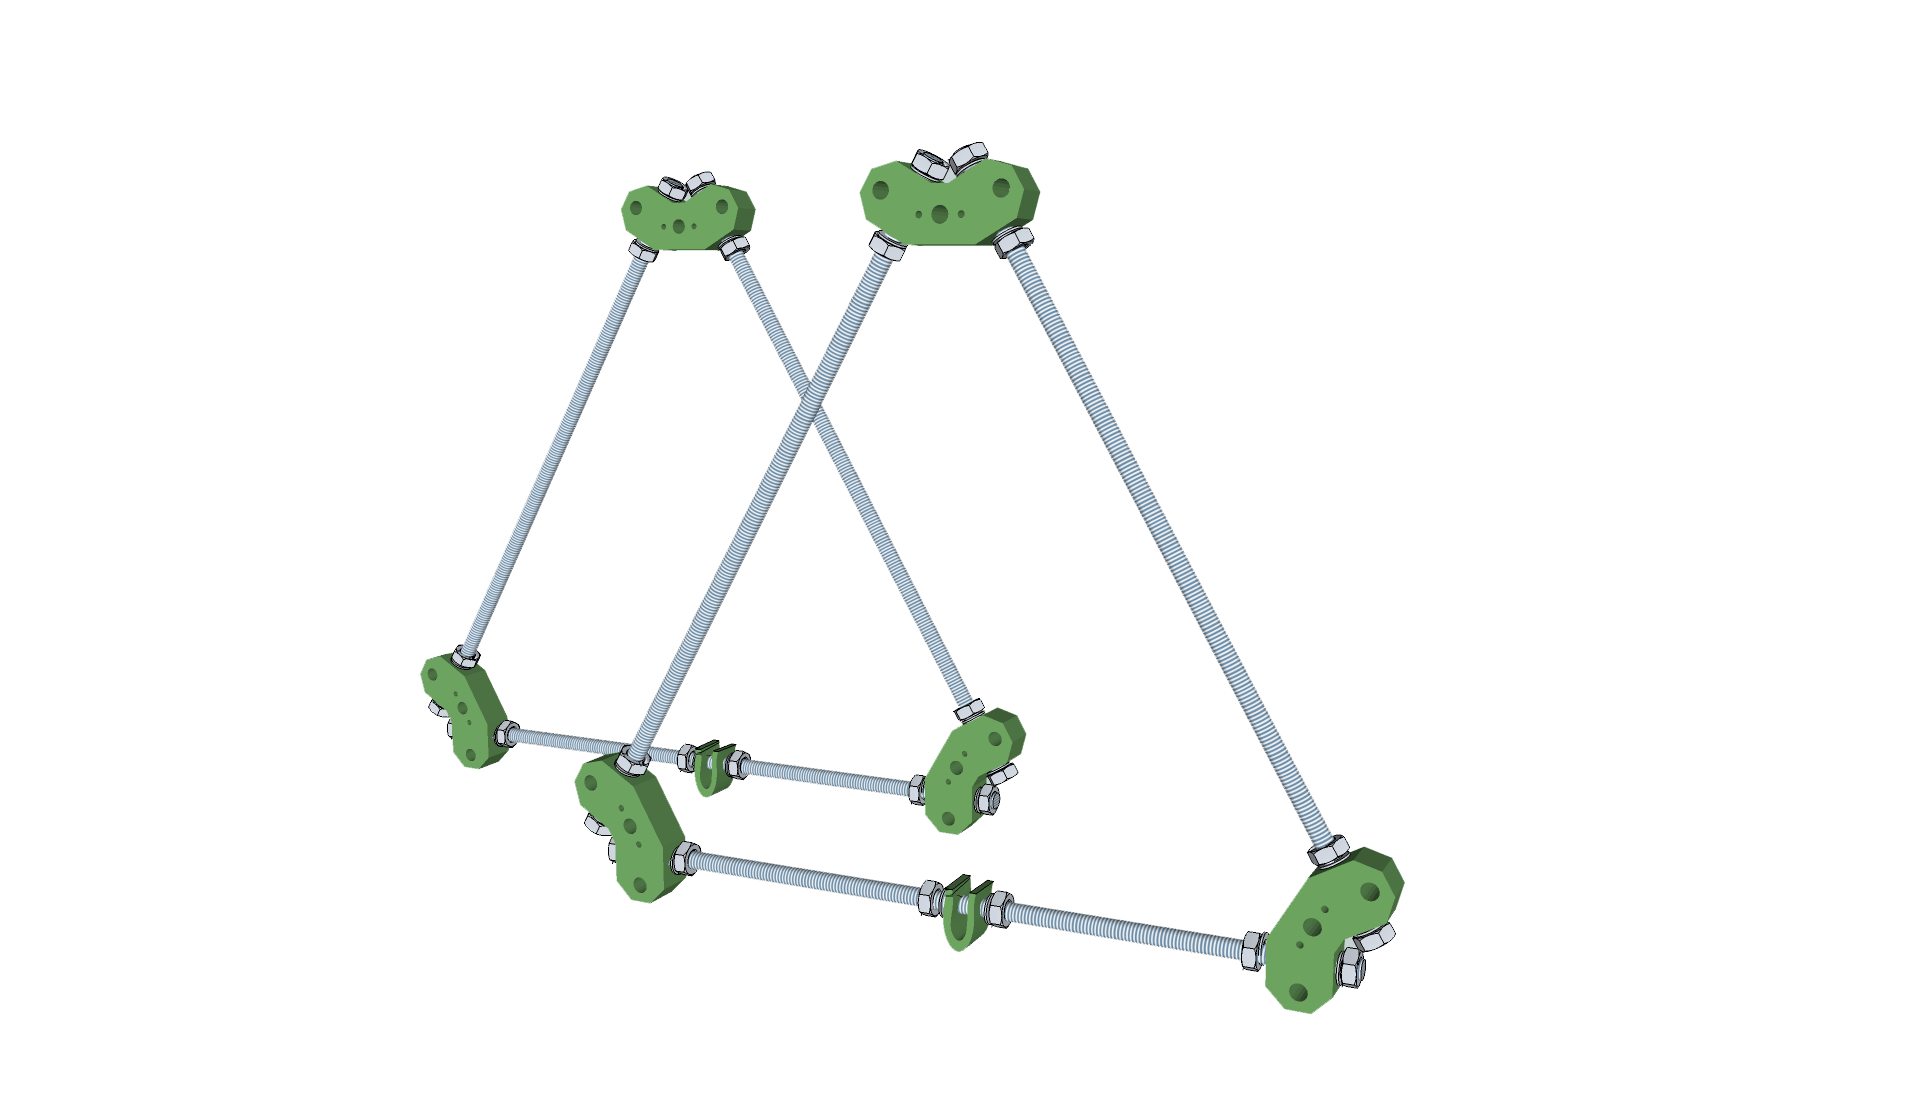
\includegraphics[width=1\linewidth]{graphics/ch1_14.png}

